\subsection{Uitwisselen van berichten}

Bij de interactie tussen twee processen moet er aan twee voorwaarden worden voldaan:

\begin{itemize}
\item Synchronisatie
\item Communicatie
\end{itemize}

Uitwisselen van berichten is een oplossing voor de tweede voorwaarde en eigenlijk ook een oplossing voor beide voorwaarden, want communicatie vereist synchronisatie. Dus als men aan communicatie voldoet men aan synchronisatie.

De feitelijke functie voor het uitwisselen van berichten wordt meestal geformuleerd als een stel primitieven:

Send(bestemming, bericht); 

Receive(bron, bericht).

\subsubsection{Synchronisatie}

Als een proces send(bestemming, bericht) doet kan het geblokkeerd worden tot het bericht ontvangen wordt of het kan ook niet worden geblokkeerd.

Als een proces receive(bron, bericht) doet, dan kan zijn er twee mogelijkheden:


\begin{enumerate}
\item Is eerder al een bericht verzonden, dan wordt het bericht ontvangen en wordt de uitvoering voortgezet.
\item Is er geen wachten bericht, dan (a) wordt het proces geblokkeerd totdat het bericht aankomt of (b) wordt het proces voortgezet en staakt het zijn poging een bericht te ontvangen.
\end{enumerate}

In de meeste systemen worden maar één of twee combinaties gebruikt:

\begin{itemize}
\item Blokkerende send en blokkerende receive, dit betekent ‘rendez-vous’.
\item Niet-blokkerende send en blokkerende receive. Dit schept de mogelijkheid om de zender meerdere berichten naar verscheidene ontvangers te sturen. De ontvangers, die wachten op hun berichten worden dan geblokkeerd totdat een bericht is aangekomen.
\end{itemize}

\subsubsection{Adressering}

De zender moet weten naar welk proces hij het bericht moest sturen. Dit kan door directe of indirecte adressering.

\textbf{Directe adressering}

Bij directe adressering bevat de primitieve send de identificatiecode van het bestemmingsproces. De primitieve receive kan op twee manieren worden behandeld. Eén mogelijkheid is te eisen dat het proces expliciet een verzendend proces aanwijst. Het proces moet dan wel van te voren weten welk proces hem een bericht gaat sturen. Bij printer-server toepassingen is het gebruiken van impliciete adressering meer effectief. In dit geval bevat de parameter bron van de primitieve receive een waarde die wordt teruggegeven wanneer de bewerking voor ontvangst is uitgevoerd.

\textbf{Indirecte adressering}

Bij indirecte adressering worden de berichten gestuurd naar wachtrijen. Deze worden ook wel postvakken genoemd. Bij een één op één communicatie en een veel op één communicatie wordt de wachtrij poort genoemd. Bij een één op veel communicatie en een veel op veel communicatie wordt de wachtrij postvak genoemd.

\subsubsection{Indeling van de berichten}

\begin{figure}[htp]
    \centering
            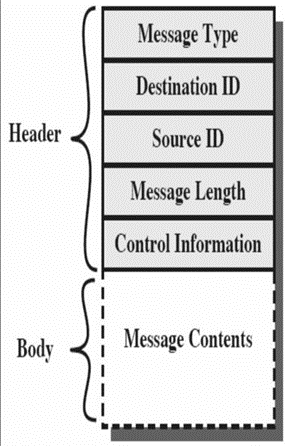
\includegraphics[width=4in]{img/indelingbericht.png}
        \caption{Indeling bericht}
    \label{fig:Indeling bericht}
\end{figure}

\subsubsection{Wederzijdse uitsluiting}

\begin{figure}[htp]
    \centering
            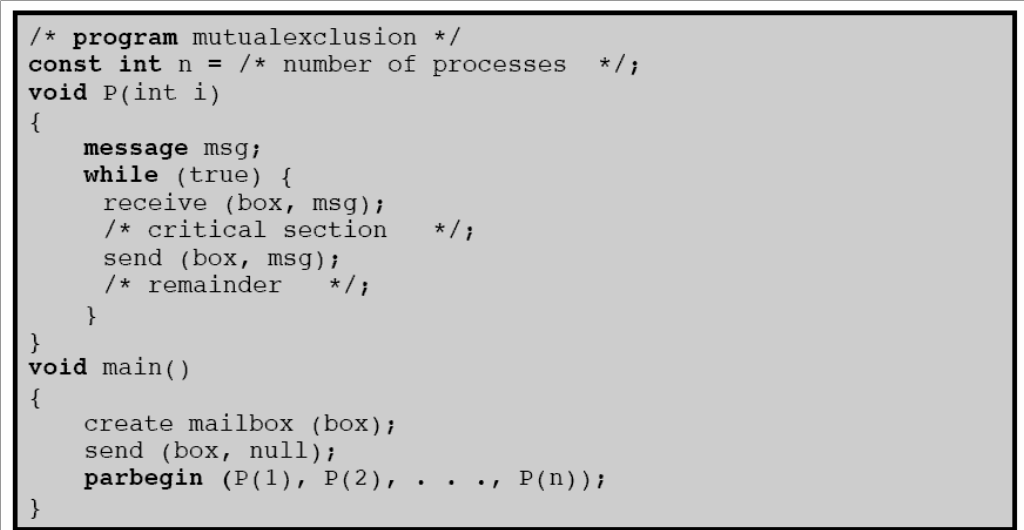
\includegraphics[width=4in]{img/mutualexclusionmessage.png}
        \caption{Indeling bericht}
    \label{fig:Indeling bericht}
\end{figure}

\begin{figure}[htp]
    \centering
            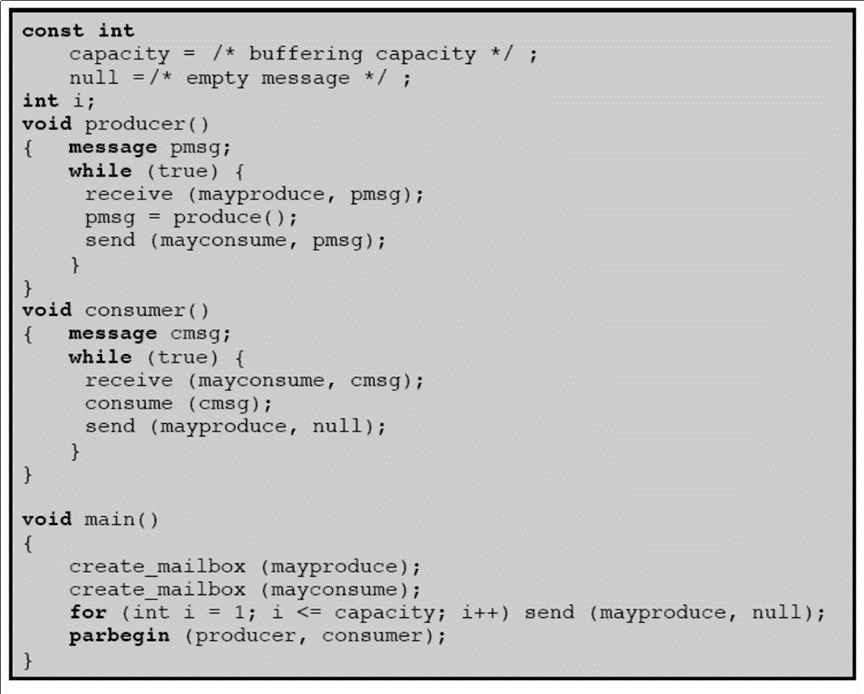
\includegraphics[width=4in]{img/producerconsumer.png}
        \caption{Indeling bericht}
    \label{fig:Indeling bericht}
\end{figure}